\section{Virtuelle Speicherverwaltung}
\label{chapVirtualMemory}
Bei der virtuellen Speicherverwaltung erfolgt die Umwandlung von vom ARM Prozessor generierten, virtuellen Adressen in physikalische Adressen durch die \ac{MMU}. Dieses Kapitel enthält die Beschreibung des Designs und der Implementierung der virtuellen Speicherverwaltung des Betriebssystems sowie der Einstellungen der MMU.\\

\subsection{Grundlegende Funktionsweise}

Die \ac{VMSAv7} definiert zwei unabhängige Formate für translation tables \cite[S. B3-1318]{ARM:ARM}:

\begin{itemize}
	\item \emph{Short-descriptor format}:
	\begin{itemize}
		\item zweistufige Seitentabelle 
		\item 32-bit Deskriptoren (PTE)
		\item 32-bit virtuelle Eingangsadresse 
		\item bis zu 40-bit große physikalische Ausgangsadresse
	\end{itemize}
	\item \emph{Long-descriptor format}:
	\begin{itemize}
		\item dreistufige Seitentabelle
		\item 64-bit Deskriptoren (\acs{PTE})
		\item verwendet \emph{Large Physical Address Extension} (LPAE)
		\item bis zu 40-bit große virtuelle Eingangsadresse 
		\item bis zu 40-bit große physikalische Ausgangsadresse
	\end{itemize}
\end{itemize}

Um die Anforderungen an das Betriebssystem zu erfüllen, reicht das zweistufige Seitentabellensystem vollkommen aus. Tabelle \ref{table:GeneralVirtualMemory} fasst die wichtigsten gegebenen Eigenschaften unter Verwendung des Short-descriptor format zusammen.\\

\begin{table}[H]
\begin{tabular}{p{7cm} | p{7cm}}
  \textbf{Eigenschaft} & \textbf{Speicherbedarf} \\ \hline
  Virtueller Speicher & 4 GB\\  
  Größe eines Page Table Entry (PTE) & 4 Byte \\
  Einträge L1 Page Table & 4096\\
  Einträge L2 Page Table & 256\\
  Speicherbedarf L1 Page Table & 4 Byte * 4096 = 16kB \\
  Speicherbedarf L2 Page Table & 4 Byte * 256 = 1kB\\
  Unterstützte Pagegrößen: & \emph{small page} (4 kB), \emph{large page} (64 kB)\\
  Unterstützte Sectiongrößen: & \emph{section} (1 MB), \emph{supersection} (16 MB)\\
 \end{tabular}
 \caption{Eigenschaften der virtuellen Speicherverwaltung der ARMv7-Architektur}
 \label{table:GeneralVirtualMemory}
\end{table}

Generiert die ARM CPU einen Speicherzugriff, wird von der MMU ein Suchlauf durchgeführt. Dieser Suchlauf wird \emph{translation table lookup} genannt. Dabei wird zuerst im \ac{TLB} nachgesehen, ob einer der 64 Einträge des TLB die zur virtuellen Adresse korrespondierende physikalische Adresse enthält. Ist dies der Fall (so genannter \emph{TLB hit}), wird der Suchlauf an dieser Stelle erfolgreich beendet.\\

Ist die angeforderte virtuelle Adresse nicht im TLB enthalten (TLB miss), wird ein page table walk durchgeführt. Das Funktionsprinzip des zweistufigen Seitentabellensystems zeigt Abbildung \ref{fig:2levelTableSystem}. Aus einem der zwei Seitentabellenregister wird die Basisadresse der darin zuvor abgelegten L1-Seitentabelle geholt. Das Format der PTE bestimmt dann, um welchen Typ von Verweis es sich handelt. Seitentabellen und ihre Einträge werden im nachfolgenden Abschnitt \ref{subsect:pageTables} genauer beschrieben.\\

\begin{figure}[H]
	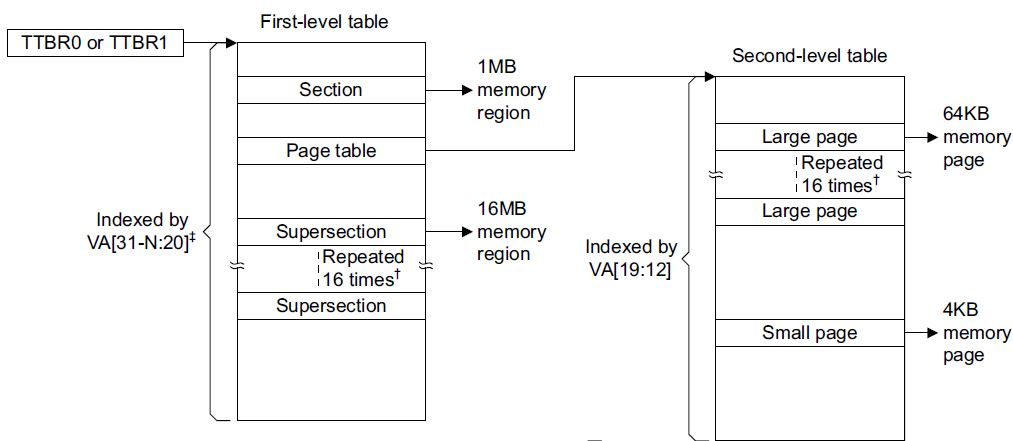
\includegraphics[scale=0.7]{chapters/mmu/figures/addressTranslation}
	\caption{Zweistufiges Seitentabellensystem \cite[S. B3-1325]{ARM:ARM}}
	\label{fig:2levelTableSystem}
\end{figure}

\vspace{2cm}
\subsubsection{Einlagerungsvorgang und Data Abort Handler}
DATA ABORT HANDLER BESCHREIBEN
\vspace{2cm}

\subsection{Umwandlung virtueller Adressen zu physikalische Adressen}

Der genaue Vorgang der Umwandlung einer vom ARM Prozessor erzeugten virtuellen Adresse in eine physikalische Speicheradresse zeigen die nachfolgenden beiden Abbildungen. Abbildung  \ref{fig:sectionTranslation} zeigt die Umwandlung einer virtuellen Adresse in die physikalische Adresse einer 1 MB Section ohne Verwendung einer L2-Seitentabelle, Abbildung \ref{fig:smallPageTranslation} diejenige einer virtuellen Adresse in ein 4 kB page frame unter Verwendung einer L2-Seitentabelle.   Die Umwandlung wird vollständig durch die Prozessor-Hardware durchgeführt.\\


\begin{figure}[H]
	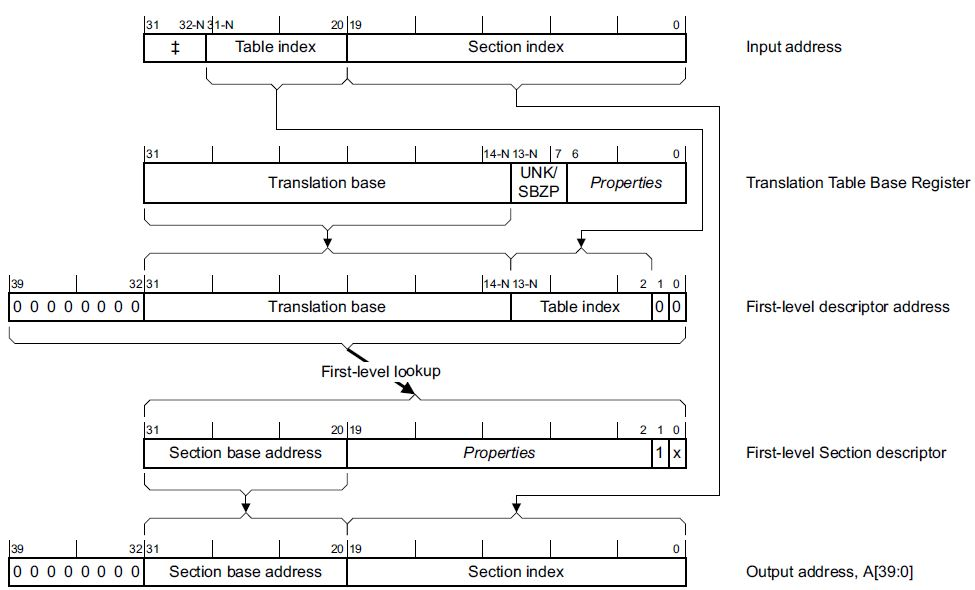
\includegraphics[scale=0.8]{chapters/mmu/figures/sectionTranslation}
	\caption{1 MB Section Translation durch die ARM CPU \cite[S. B3-1335]{ARM:ARM}}
	\label{fig:sectionTranslation}
\end{figure}

\begin{figure}[H]
	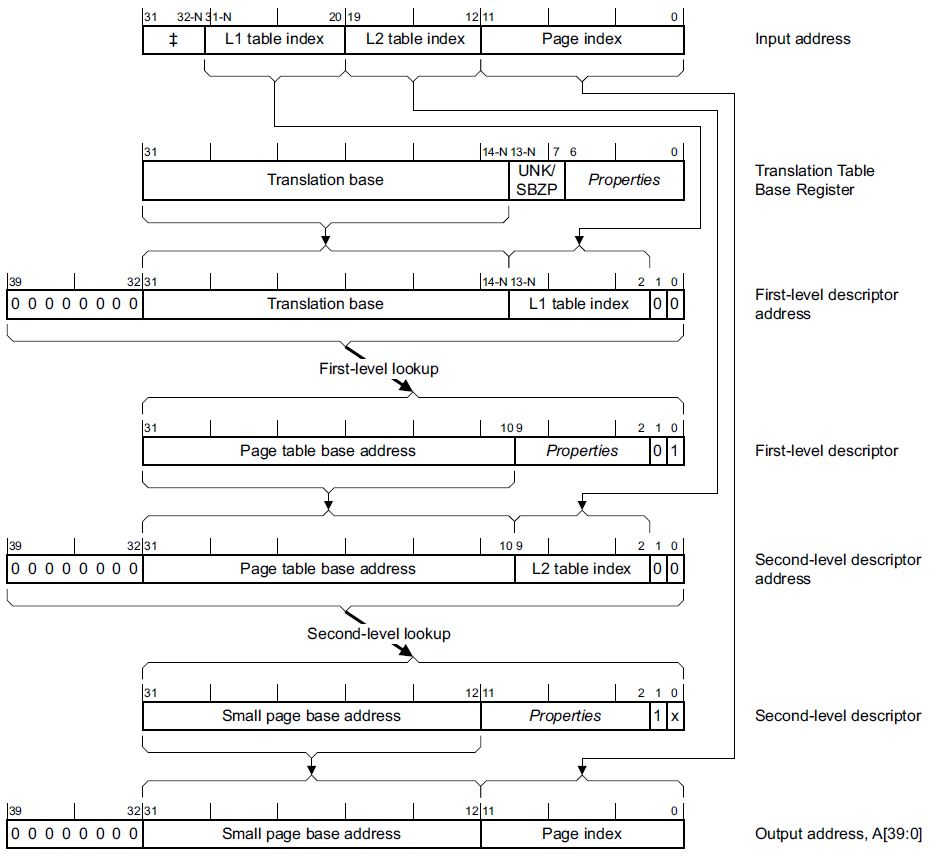
\includegraphics[scale=0.8]{chapters/mmu/figures/smallPageTranslation}
	\caption{Small Page Translation durch die ARM CPU \cite[S. B3-1337]{ARM:ARM}}
	\label{fig:smallPageTranslation}
\end{figure}

\subsection{Seitentabellen und Seitentabelleneinträge}
\label{subsect:pageTables}

Der verwendete ARM Prozessor verfügt über zwei Register (\acf{TTBR}, \emph{TTBR0} und \emph{TTBR1}), welche Startadressen von Seitentabellen enthalten  \cite[S. B3-1320]{ARM:ARM}. Ihre Formate sind nahezu identisch und in den Abbildungen \ref{fig:TTBR0Format} und \ref{fig:TTBR1Format} zu sehen. Diese Register übernehmen im Betriebssystem die folgende Funktion:

\begin{itemize}
	\item TTBR0: Wird für prozessspezifische Adressen verwendet. Jeder Prozess enthält bei seiner Initialisierung eine eigene L1-Seitentabelle. Bei einem Kontextwechsel erhält das TTBR0 eine Referenz auf L1-Seitentabelle des neuen Kontextes/Prozesses.
	\item TTBR1: Wird für das Betriebssystem selbst und für memory-mapped I/O verwendet. Diese ändern sich bei einem Kontextwechsel nicht.
\end{itemize}


\begin{figure}[H]
	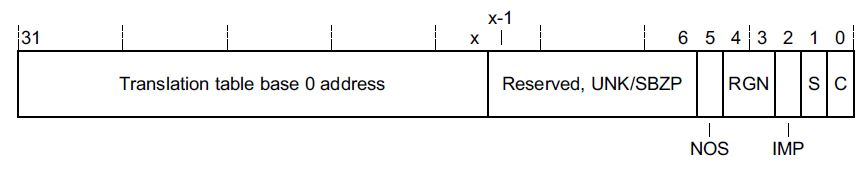
\includegraphics[scale=0.8]{chapters/mmu/figures/ttbr0format}
	\caption{TTBR0 Format \cite[S. B4-1726]{ARM:ARM}}
	\label{fig:TTBR0Format}
\end{figure}


\begin{figure}[H]
	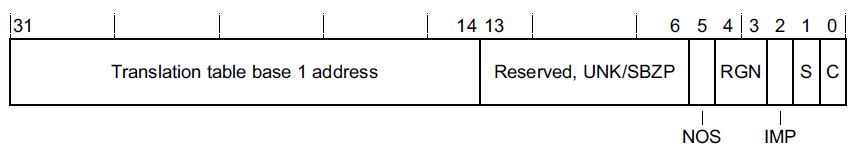
\includegraphics[scale=0.8]{chapters/mmu/figures/ttbr1format}
	\caption{TTBR1 Format \cite[S. B4-1730]{ARM:ARM}}
	\label{fig:TTBR1Format}
\end{figure}

Das Beschreiben der Seitentabellenregister erfolgt, wie bei nahezu jeder MMU-Funktionalität, mittels Assemblerbefehlen, die auf die CP15 Coprozessor Register zugreifen.\\

Beim Füllen der Seitentabellen sind vorgegebene Formate für die beiden Typen von Deskriptoren unbedingt zu beachten. Die Abbildungen \ref{fig:firstLevelDescriptor} und \ref{fig:secondLevelDescriptor} fassen die Formate für first-level und second-level Deskriptoren zusammen. Beiden Deskriptortypen gleich ist die vorgeschriebene Länge von 32 Bit.\\

\subsubsection*{First-level Deskriptoren}

Die First-Level Deskriptortypen werden auf folgende Weise verwendet:

\begin{itemize}
	\item sections für die \ac{MPT} (siehe Abschnitt \ref{subsect:memoryMapping}) 
	\item page table für L1-Seitentabellen von Prozessen (siehe Abschnitt \ref{subsect:memoryMapping})
\end{itemize}

Für die Erstellung von first-level Deskriptoren wurde eine Struktur erstellt, welche in Listing \ref{codeFirstLevelDescriptor} aufgeführt ist. Diese Struktur und jene des second-level Deskriptors wird bei den nachfolgenden Erläuterungen zur MMU benötigt.\\

\begin{figure}[H]
	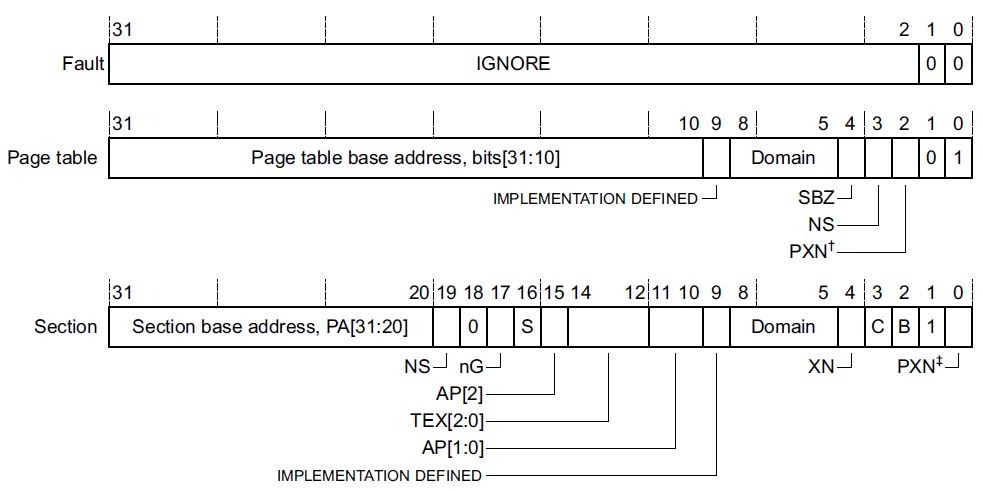
\includegraphics[scale=0.7]{chapters/mmu/figures/firstLevelDescriptor}
	\caption{First-Level Deskriptorformate \cite[S. B3-1326]{ARM:ARM}}
	\label{fig:firstLevelDescriptor}
\end{figure}


\lstinputlisting[language=C, caption=Struktur für first-level Deskriptoren, captionpos=b, label=codeFirstLevelDescriptor]{chapters/mmu/codefiles/firstLevelDescriptor.c}

\subsection*{Second-level Deskriptoren}

In der Speicherverwaltung des Betriebssystems werden ausschließlich small pages verwendet. Ausschlaggebende Gründe, warum small pages den Vorzug gegenüber large pages erhielten, sind die folgenden:

\begin{itemize}
	\item small pages müssen nur einmal in die L2-Seitentabelle eingetragen werden, large pages hingegen 16 mal
	\item L1- und L2-Seitentabellen, die 16 kB bzw. 1 kB Speicher benötigen, belegen bei ihrer Erzeugung nur vier volle page frames bzw. ein page frame physikalischen Speichers zu einem Viertel. Dadurch wird die Speicherfragmentierung verglichen mit large pages stark verringert
\end{itemize}

Die Zusammensetzung der Struktur für second-level Deskriptoren ist in Listing \ref{codeSecondLevelDescriptor} dargestellt.\\

\begin{figure}[H]
	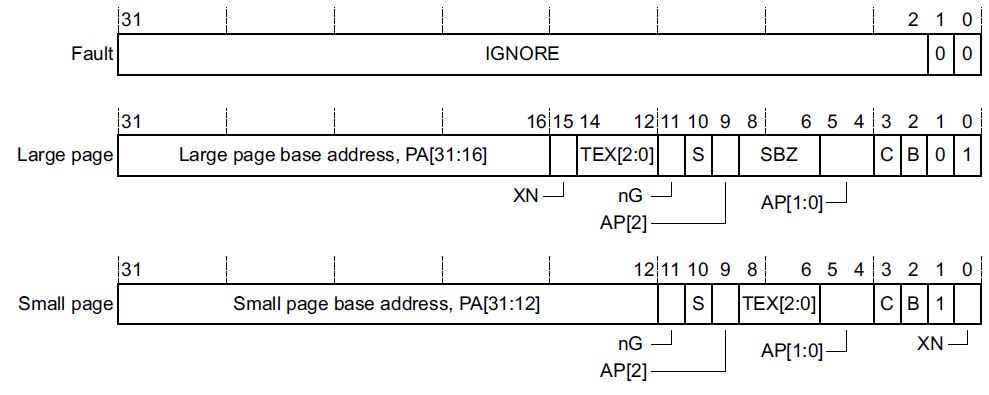
\includegraphics[scale=0.7]{chapters/mmu/figures/secondLevelDescriptor}
	\caption{Second-Level Deskriptorformate \cite[S. B3-1327]{ARM:ARM}}
	\label{fig:secondLevelDescriptor}
\end{figure}


\lstinputlisting[language=C, caption=Struktur für second-level Deskriptoren, captionpos=b, label=codeSecondLevelDescriptor]{chapters/mmu/codefiles/secondLevelDescriptor.c}


\subsection{Aufteilung des virtuellen Speichers und Mapping}
\label{subsect:memoryMapping}

Die Speicherverwaltung des Betriebssystems kann Abbildung \ref{fig:MemoryMap} entnommen werden. Die rechte Seite stellt das physikalische Speichermapping dar und wurde dem Datenblatt des ARM \cite[S. 155]{ARM:TRM} entnommen. Die linke Seite zeigt die Aufteilung des virtuellen Speichers.\\

Organisiert ist der virtuelle Speicher in Speicherregionen. Eine zusätzliche Aufteilung betrifft die Zuständigkeitsbereiche für die Seitentabellenregister TTBR0 und TTBR1. Der ARM Cortex-A8 bietet die Möglichkeit, den virtuellen Speicher in einen \emph{Prozessbereich} und einen \emph{Kernelbereich} aufzuteilen. Der Prozessbereich enthält dabei alle virtuellen Adressen, die für Prozesse zugänglich sind. Der Kernelbereich enthält Komponenten, die sich bei Prozesswechseln nicht ändern. Dazu zählen das Betriebssystem selbst sowie die memory-mapped I/O. \\ 

Die Einstellungen zur Aufteilung des virtuellen Speichers werden im  TTBCR (Translation Table Base Control Register) vorgenommen. Die möglichen Aufteilungsbereiche finden sich in Tabelle B3-1, \cite[S. B3-1330]{ARM:ARM}.\\

Physikalisch steht 1 GB Speicher für die page frames zur Verfügung. Dieser wird im virtuellen Speicher an die Adressen 0x00000000 bis 0x3FFFFFFF gemapped. Die Komponenten der Kernelregion, die sich bei Prozesswechseln nicht ändern, beginnen bei Adressen ab 0x40000000. Damit ergibt sich eine Aufteilung des virtuellen Speichers, wie sie in Abbildung \ref{fig:MemoryMap} dargestellt ist, mit der Bereichsgrenze 0x40000000.\\

Die Adressen ab der Bereichsgrenze bis zu den vollen 4 GB virtuellem Speicher bei der Adresse 0xFFFFFFFF werden in eine so genannte L1 \ac{MPT} gemapped. Bei der Aktivierung der MMU wird die Adresse dieser master page table in das Register TTBR1 geschrieben. Danach wird TTBR1 während der Laufzeit des Betriebssystems nicht mehr verändert.\\

Bei der Initialisierung eines Prozesses wird für den Prozess eine L1 page, die den Prozessbereich abdeckt, angelegt. Soll ein Prozess zur Ausführung gebracht werden, muss seine L1 page table in das TTBR0 geschrieben werden. Das TTBR0 muss zur Laufzeit des Betriebssystems bei Kontextwechseln von Prozessen aktualisiert werden.\\


\begin{figure}[H]
	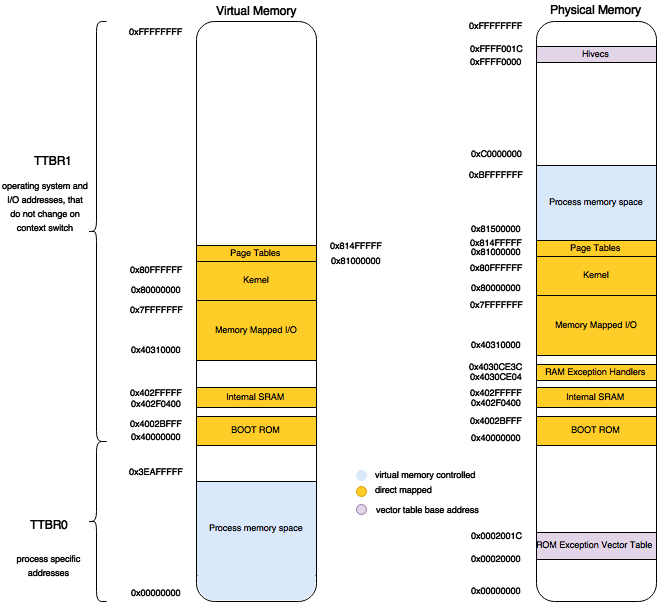
\includegraphics[scale=0.60]{chapters/mmu/figures/MemoryMap}
	\caption{Memory Map des Betriebssystems}
	\label{fig:MemoryMap}
\end{figure}




\begin{table}[H]
\begin{tabular}{p{7cm} | p{7cm}}
  \textbf{Eigenschaft} & \textbf{Beschreibung} \\ \hline
  Größe der Pages & 4 kB\\
  Virtueller Speicher für Prozesse & 1003 MB\\
  Max. Anzahl von L1 und L2 Page Tables & 320 L1 Page Tables oder 1 L1 Page Table + 1276 L2 Page  Table\\
  Theoretisch Max. Anzahl von Prozessen & 320\\
 \end{tabular}
 \caption{Eigenschaften der virtuellen Speicherverwaltung des OS}
 \label{table:SpecifiedVirtualMemory}
\end{table}

\subsubsection{Speicherregionen}

Das nachfolgende Listing \ref{codeMemoryRegion} zeigt die Struktur, mit welcher Regionen im virtuellen Speicher erstellt und verwaltet werden. Sie bieten die Möglichkeit, unterschiedlich große Bereiche des virtuellen Speichers mit denselben Eigenschaften und Zugriffsrechten zu versehen.\\

Erstellt werden solche Speicherregionen sämtliche in Abbildung \ref{fig:MemoryMap} gezeigten Bereiche. Sie enthalten die virtuelle Anfangs- und Endadresse der Region sowie Pagegröße und Zugriffsrechte auf die Region. Weiters enthalten sie eine verkettete Liste von Strukturen, die den Status(reserviert oder nicht reserviert) der einzelnen Pages verwaltet.\\

\lstinputlisting[language=C, caption=Struktur für die Verwaltung von Speicherregionen, captionpos=b, label=codeMemoryRegion]{chapters/mmu/codefiles/region.c}
\vspace{0.5cm}

Zusammengefasst dargestellt sind in Tabelle \ref{table:MemoryRegions} alle Speicherregionen des Betriebssystems. Ein direktes Mapping bedeutet dabei, dass die virtuelle Adresse der physikalischen entspricht.\\

\begin{table}[H]
\begin{tabular}{p{4cm} | p{1.5cm} | p{1.5cm} | p{6cm}}
  \textbf{Region} & \textbf{Mapping} & \textbf{Größe} & \textbf{Beschreibung} \\ \hline
  Page Tables & direkt & 5 MB & Speicherort für L1 und L2 page tables\\
  Kernel & direkt & 16 MB & Speicherort für das Betriebssystem\\
  Memory-Mapped I/O & direkt &  1 GB & Peripheriemodule\\
  Exception Handlers & direkt &  4 kB & Enthält die Exception vector table\\
  Internal SRAM & direkt & 64 kB & Enthält die Exception handler\\
  BOOT ROM & direkt & 192 kB & für zukünftige Erweiterungen \\ 
  Process memory space & virtuell & 1 GB & Speicherbereich für Prozesse
 \end{tabular}
 \caption{Angelegte Speicherregionen}
 \label{table:MemoryRegions}
\end{table}


\subsubsection{Master Page Table}

Um das Mapping der \ac{MPT} verstehen zu können, wird nochmals auf den Adresstranslationsablauf in Abbildung \ref{fig:sectionTranslation} verwiesen. Alle direkt gemappten Regions aus Tabelle \ref{table:MemoryRegions} werden in die L1 \ac{MPT} als 1 MB Sections gemapped.\\

Die Adresse eines Eintrags in der page table setzt sich zusammen aus der Basisadresse der entspreche page table und einem Index. Nach dem setzen der Attribute des page table Eintrags wird durch die Funktion \emph{mmuGetTableIndex} aus den obersten Bits der physikalischen Adresse der Intex in der page table berechnet. Der Index muss um 2 bit nach links geshiftet werden, um das Alignment von 4 Byte einzuhalten. Schließlich wird der geshiftete Index noch durch die Datentypgröße von 4 Byte geteilt. Damit wird die korrekte Adresse des zu schreibenden Tabelleneintrags durch Pointerarithmetik ermittelt. An diese Adresse wird nun der Eintrag geschrieben, der zuvor durch die Funktion \emph{mmuCreateL1PageTableEntry} aus der übergebenen first-level Deskriptorstruktur erstellt wurde. Listing \ref{codeMasterPageTableMapping} zeigt die praktische Ausführung des direkten Mappings in die \ac{MPT}.\\ 


\lstinputlisting[language=C, caption=Funktion für direktes Mapping in die master page table, captionpos=b, label=codeMasterPageTableMapping]{chapters/mmu/codefiles/directMapIntoMasterPageTable.c}

\subsection{Allokierung der Page Frames}

Für die Verwaltung der page frames wurde eine Bitsmap verwendet. Abbildung \ref{fig:BitsMap} zeigt das Prinzip.
Die Bitsmap wird durch ein Array der Länge N/8 Bytes realisiert. N steht hier für die Anzahl der page frames. Das i-te Bit im n-ten Byte der Bitsmap definiert den Verwendungsstatus des (n*8 + i) –ten page frame.




\begin{figure}[H]
	\centering
	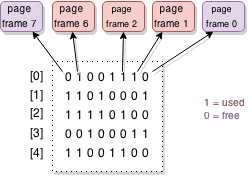
\includegraphics[scale=1]{chapters/mmu/figures/BitsMap}
	\caption{Beispiel einer Bitsmap zur Verwaltung der Page Frames}
	\label{fig:BitsMap}
\end{figure}

\subsubsection{Allokation von Page Frames bei Data Abort Exception}

\subsection{Aktivieren der MMU}
\label{subsect:activateMMU}

Bevor die MMU erfolgreich aktiviert werden kann, muss vorher eine Reihe von Einstellungen gesetzt werden.\\


Listing \ref{codeMMUInit} zeigt den kompletten Ablauf zur Aktivierung der MMU.

\lstinputlisting[language=C, caption=Aktivierung der MMU, captionpos=b, label=codeMMUInit]{chapters/mmu/codefiles/MMUInit.c}


\subsection{Interaktion der MMU mit Prozessen}

Die Schnittstelle der Softwareimplementierung der MMU zeigt Listing \ref{codeMMUFunctions}.\\

\lstinputlisting[language=C, caption=Softwareschnittstelle der MMU, captionpos=b,  label=codeMMUFunctions]{chapters/mmu/codefiles/MMUFunctions.c}
\vspace{0.5cm}

Die Schnittstellenfunktionen werden auf die folgende Weise verwendet: 

\begin{description}
	\item[MMUInit] \hfill \\ Initialisiert die Regionen des virtuellen Speichers und die MMU für die Verwendung. Nach dem Ausführen dieser Funktion ist die MMU eingeschaltet. Bei nach erfolgreichem Ausführen wird als Rückgabewert 1 zurückgeliefert. Diese Funktion wird bei der Initialisierung des Prozess Managers aufgerufen.
	\item[MMUSwitchToProcess] \hfill \\ Bringt den als Parameter übergebenen Prozess zur Ausführung. Dabei wird der TLB geflusht und die Adresse der L1 page table des Prozesses in das TTBR0 geschrieben. 
	\item[MMUInitProcess] \hfill \\ Erstellt beim Erzeugen eines neuen Prozesses eine L1 page table für diesen Prozess. Die page table wird mit fault entries initialisiert.
	\item[MMUHandleDataAbortException] \hfill \\ Diese Funktion wird bei jeder Data Abort Exception ausgeführt. Sie wird durch einen in Assembler implementierten Dabt Handler aufgerufen. Die Funktion lädt die virtuelle Adresse, bei deren Zugriff die Data Abort Exception ausgelöst wurde aus dem \acf{DFAR} sowie den Fehlerstatus aus dem \acf{DFSR}. Die weitere Vorgehensweise wird in Abhängigkeit vom Fehlerstatus durchgeführt.
	\item[MMUFreeAllPageFramesOfProcess] \hfill \\ Beim Killen eines Prozesses gibt diese Funktion sämtliche von diesem Prozess belegten page frames in der zur Verwaltung der page frames eingesetzten Bitsmap wieder frei.
\end{description}

\pagebreak 